\documentclass{article}
\usepackage[utf8]{inputenc}
\usepackage{listings}
\usepackage{CJKutf8}
\usepackage{amsmath}
\usepackage{amssymb}
\usepackage{graphicx}
\usepackage{algorithm}
\usepackage{algpseudocode}
\usepackage{float}
\usepackage{tikz}
\usepackage{url}
\usetikzlibrary{trees}

\title{DSA HW2}
\author{b09901142 EE3 呂睿超}
\date{May 2023}

\usepackage{xcolor}

\definecolor{codegreen}{rgb}{0,0.6,0}
\definecolor{codegray}{rgb}{0.5,0.5,0.5}
\definecolor{codepurple}{rgb}{0.58,0,0.82}
\definecolor{backcolour}{rgb}{0.95,0.95,0.92}

\lstdefinestyle{mystyle}{
    backgroundcolor=\color{backcolour},   
    commentstyle=\color{codegreen},
    keywordstyle=\color{magenta},
    numberstyle=\tiny\color{codegray},
    stringstyle=\color{codepurple},
    basicstyle=\ttfamily\footnotesize,
    breakatwhitespace=false,         
    breaklines=true,                 
    captionpos=b,                    
    keepspaces=true,                 
    numbers=left,                    
    numbersep=5pt,                  
    showspaces=false,                
    showstringspaces=false,
    showtabs=false,                  
    tabsize=2
}

\lstset{style=mystyle}

\begin{document}
\begin{CJK*}{UTF8}{bsmi}
\maketitle

\section{Problem 1 - Birds Playing in the tree.}
\textbf{All problems in this section without specifically showing references are done all by myself}

\begin{enumerate}
    \item The figure below is a sample tree.
    \begin{figure}[h]
     \begin{tikzpicture}[level distance=1.5cm,
  level 1/.style={sibling distance=3cm},
  level 2/.style={sibling distance=1.5cm}]
  \node {$n_{2}$}
    child {node {$n_{3}$}
      child {node {$n_{0}$}}
      child {node {$n_{0}$}}
      child {node {$n_{0}$}}
    }
    child {node {$n_{2}$}
    child {node {$n_{0}$}}
      child {node {$n_{2}$}
      child{node{$n_{0}$}}
          child{node{$n_{0}$}
          }}
    };
\end{tikzpicture}
\end{figure}
We can see that if we repeatedly count all nodes with degrees larger than 1(in this case 2+3+2+2,which is $n_2$*3 + $n_3$*1), we need to minus the nodes that both have parents and children.(In this case, $n_2$ = 3,$n_3$ = 1,but root don't have parent)
Therefore, we can find out the pattern,\\
$n_0 = (\sum_{i=1}^{k} n_i*i - \sum_{i=1}^{k} {n_i}) + 1 (root)$\\
$ = \sum_{i=1}^{k} {n_i*(i-1)} + 1$
   

    \item ref: \url{https://www.geeksforgeeks.org/construct-tree-from-given-/inorder-and-preorder-traversal/} 
    \begin{enumerate}
        \item The preorder traversal implies that the leftmost element of certain sequence is the root of the subtree.(the leftmost element of the whole traversal is the root of the tree.)
        \item After identifing the root, we can distinguish the left subtree and right subtree by the inorder traversal since the left subtree must be on the left of root and vice versa.
        \item In this question, I use the following figure to demonstrate (a) and (b)
        \begin{figure}[h]
            \centering
            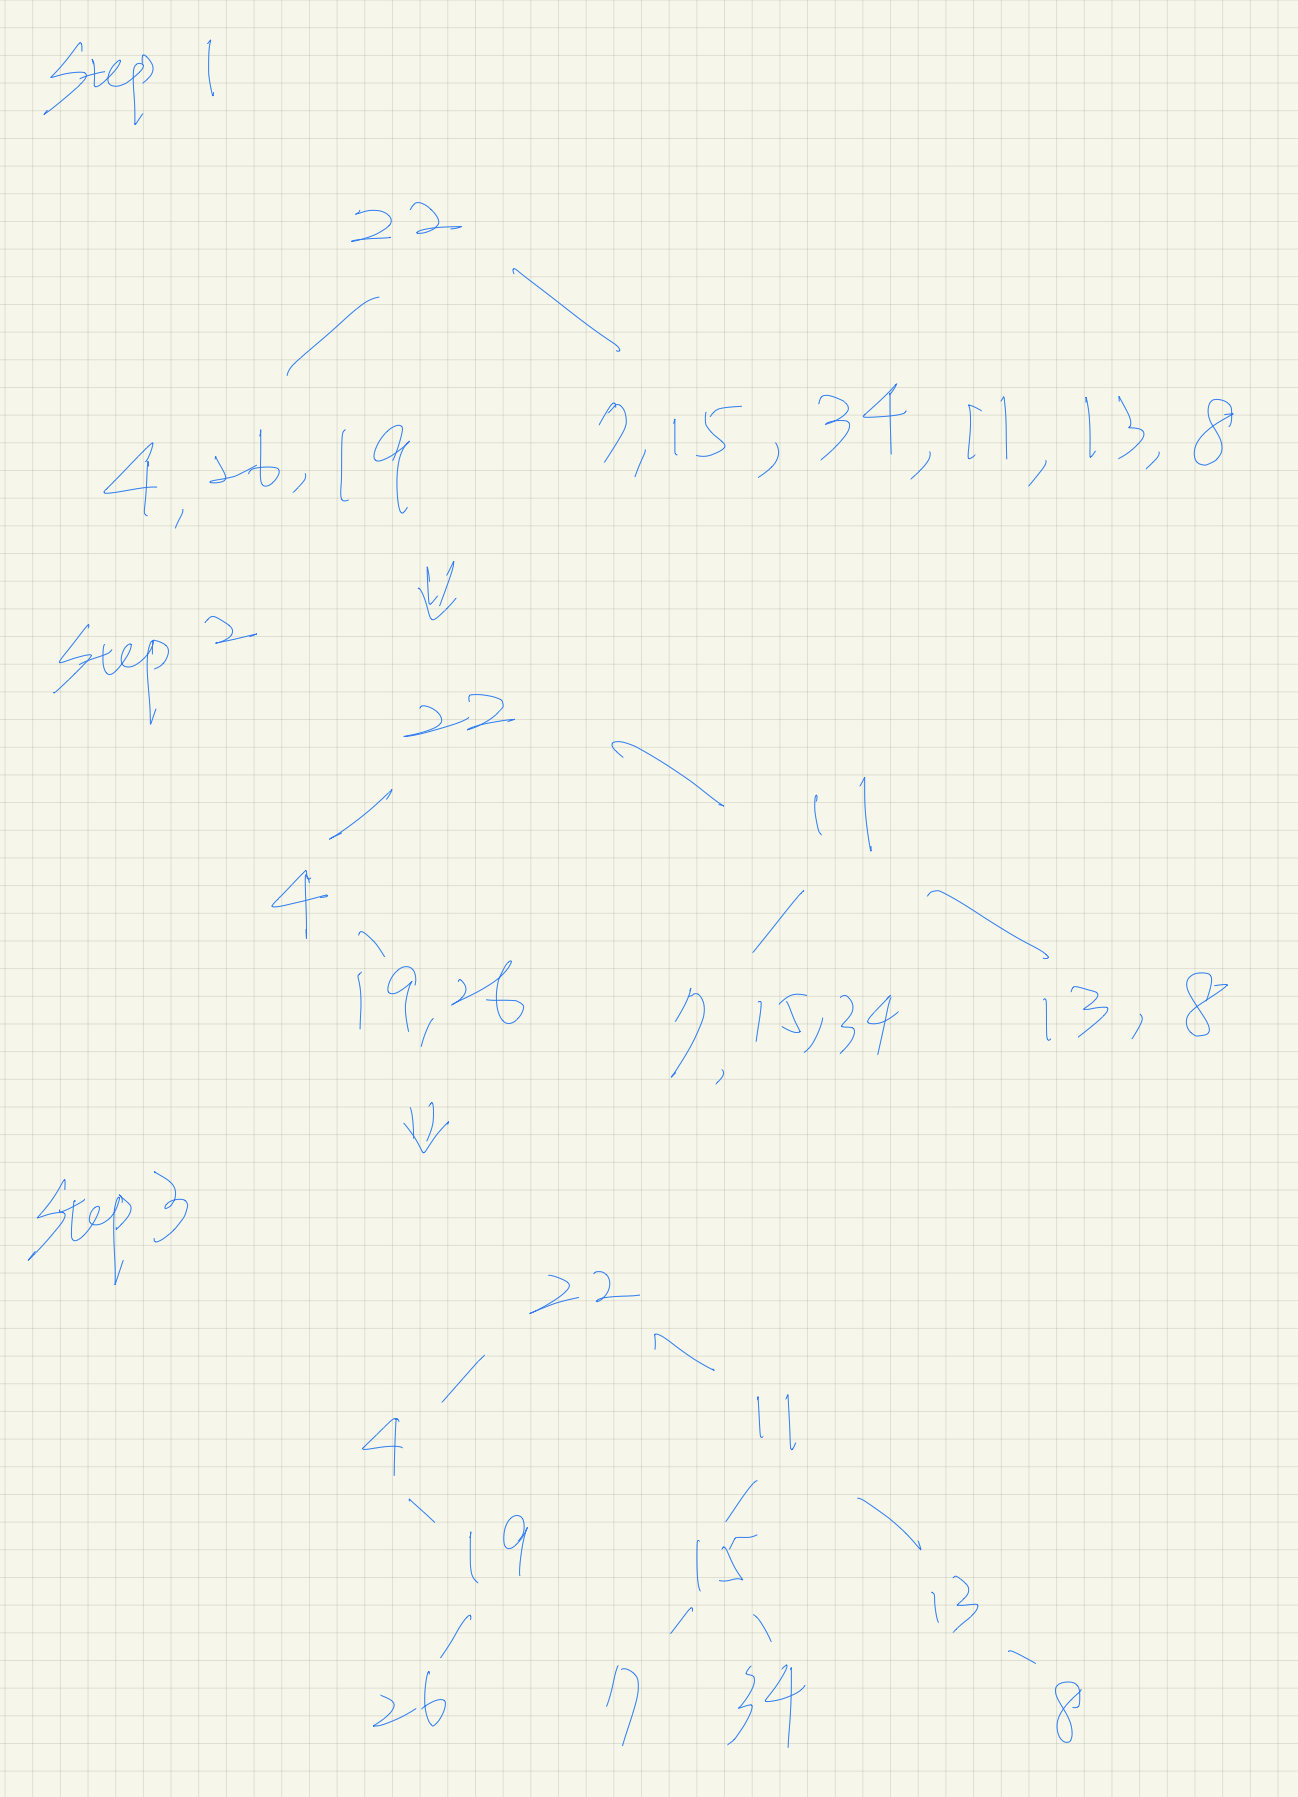
\includegraphics[width=0.4\textwidth]{IMG_0255.jpg}
            \caption{Construct Unique tree}
            \label{fig:my_label}
        \end{figure}
    \end{enumerate}
    
    
    

    \item We can't construct an \textbf{unique} binary tree with given only preorder and postorder traversals.
    \begin{enumerate}
        \item Preorder traversal traverses in the sequence : center - left - right
        \item Postorder traversal traverses in the sequence : left - right - center 
        \item From (a),(b) we can conclude that we can't distinguish the distribution of elements in left subtree and right subtree since there isn't an element to seperate them as in the previous question.
        \item Figure 2 is an counterexample that there could be two possible binary trees that satisfy both traversal orders.
        \begin{figure}[h]
            \centering
            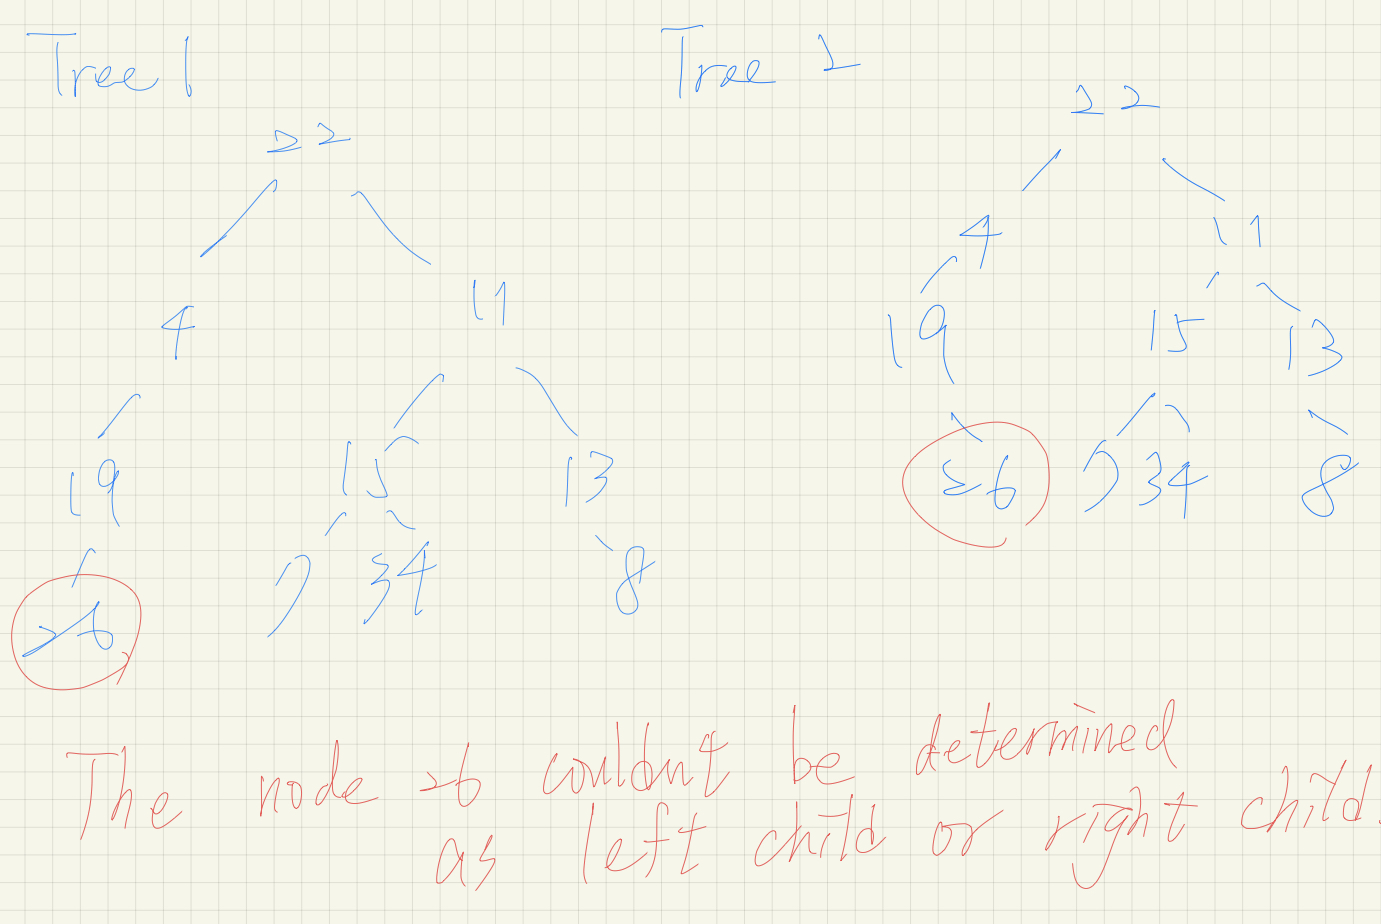
\includegraphics[width=0.4\textwidth]{IMG_0256.jpg}
            \caption{Construct Unique tree}
            \label{fig:my_label}
        \end{figure}

    \end{enumerate}
    \item The BST is as the figure below.
    \begin{figure}[h]
     \begin{tikzpicture}[level distance=1.5cm,
  level 1/.style={sibling distance=3cm},
  level 2/.style={sibling distance=1.5cm}]
  \node {26}
    child {node {$8$}
      child {node {$7$}
      child[left]{node{1}}}
      child {node {$12$}}
    }
    child {node {$52$}
    child {node {$34$}}
      child {node {76}
          child[right]{node{89}
          }}
    };
\end{tikzpicture}
\end{figure}

    \item The psuedo code is as below
    \begin{algorithm}[H]
        \caption{Construct\_BST(arr,left,right)}
        \begin{algorithmic}
        \While{left$<$right}
        \State mid = (left+right)//2
    \State Left\_subtree = Construct\_BST(arr[left:mid],left,mid) \Comment{arr[left]~arr[mid-1]}
        \State Right\_subtree = Construct\_BST(arr[mid+1:right],mid+1,right)      
        \EndWhile
        \end{algorithmic}
        \end{algorithm}
    \begin{algorithm}[H]
        \caption{Main()}
        \begin{algorithmic}
         \State Construct\_BST(arr,0,arr.length)
        \end{algorithmic}
    \end{algorithm}

\item 
    \begin{enumerate}
        \item Time complexity of Pigeon's\_Store is O(MP) since it just stores each character one by one.
        \item Extra space complexity of Pigeon's\_Store is O(MP) since it requires the M by P array \textit{bugs} that it declared.
        \item Time complexity of Pigeon's\_Search is O(NMP) since it just traverse through each element by simply going through all rows and columns(O(MP)). Also,it needs to search all N bugs(O(N)). 
        \item Extra space complexity of Pigeon's\_Search is O(N) since it requires the length-N array \textit{eat} that it declared.
    \end{enumerate}
\item 
    \begin{enumerate}
        \item Time complexity of Spotteddove's\_Store is O(MP) since it also just stores each character one by one.
        \item Extra space complexity of Spotteddove's\_Store is O($26^P$) since the tree\ textit{bugsRoot} requires 26 links at each node and it requires P levels.
        \item Time complexity of Spotteddove's\_Search is O(NP) since it just traverse through each element by going through each level of the tree(O(P)). Also,it needs to search all N bugs(O(N)). 
        \item Extra space complexity of Spotteddove's\_Search is O(N) since it requires the length-N array \textit{eat} that it declared.
    \end{enumerate}
\item If it is a situation with limited memory but loose limit on operting time, I would choose pigeon's algorithm over spotteddoves' since we can see the difference in the extra space complexity that we have analyzed.
\end{enumerate}

\section{Problem 2 - Valorant}
\textbf{All problems in this section are done all by myself}
\begin{enumerate}
    \item Step 1 : 7,3,5,0,2,8,6,1; Step 2 : 7,3,5,0 $||$ 2,8,6,1; \\
          Step 3 : 7,3 $||$ 5,0 $||$ 2,8 $||$ 6,1; Step 4: 7 $||$ 3 $||$ 5 $||$ 0 $||$ 2 $||$ 8 $||$ 6 $||$ 1;\\
          Step 5 : 3,7 $||$ 0,5 $||$ 2,8 $||$ 1,6; Step 6: 0,3,5,7 $||$ 1,2,6,8;\\
          Step 7 : 0,1,2,3,5,6,7,8
    
    \item  I used brute force to calculate by directly inspecting through all possible pairs. Considering 6(r[0]),
    the pairs that are reversions are (6,5),(6,2),(6,0),(6,5),(6,1) (5 reversions). After considering all pairs, I got 5+3+5+2+1+1 = 17 reversions.
  
    \item \begin{enumerate}
        \item Algorithm as below 
        \begin{algorithm}[H]
        \caption{Count\_Rev\_by\_Merge(arr,p,r)}
        \begin{algorithmic}
        \State 
        \If{p $<$ r}
            \State q = floor((p+r)/2)
            \State temp1 = Count\_Rev\_by\_Merge(arr,p,q)
            \State temp2 = Count\_Rev\_by\_Merge(arr,q+1,r)
            \State temp3 = Merge(arr,p,q,r)
        \EndIf
        \State \Return temp1+temp2+temp3
        \end{algorithmic}
        \end{algorithm}
        \begin{algorithm}[H]
        \caption{Merge(arr,p,q,r)}
        \begin{algorithmic}
        \State Copy arr[p,..,q],arr[q+1,..,r] to extra space array L and R
        \State i,j = 1,1
        \State ans = 0
        \State left\_length = q-p+1, right\_length =  r-q
        \For{k = p to r}
            \If{L[i] $<$ R[j]}
                \State arr[k] = L[i]
                \State i = i+1
                \State left\_length = left\_length -1
            \Else
                \State arr[k] = R[j]
                \State j = j+1
                \State right\_length = right\_length -1
                \State ans = ans + left\_length 
            \EndIf
        \EndFor
        \State \Return new
        \end{algorithmic}
        \end{algorithm}
        \begin{algorithm}[H]
        \caption{Main()}
        \begin{algorithmic}
         \State ans = Count\_Rev\_by\_Merge(arr,0,arr.length)
         \Return ans
        \end{algorithmic}
        \end{algorithm}
        
        \item Correctness : In the circumstance of R[j] $>$ L[i], putting R[j] back to arr[k] is the operation of swapping R[j] to the left of the items that is left in L(because they haven't been sorted). Also a reversion implies a position relationship that the smaller element is on the right of the larger element.
        Therefore, counting the swaps in merge sort is equivalent to counting the reversions.
        \item Time Complexity = O(${n log{n}}$), Space complexity = O(n) , this algorithm simply relies on merge sort. The time and space complexity in proven in class or in the textbook.
    \end{enumerate}
        
    \item  \begin{enumerate}
        \item Algorithm as below
        \begin{algorithm}[H]
        \caption{Possible\_Candidate(data)}
        \begin{algorithmic}
        \State Sort(data) with any sorting method with time complexity O(n$log{n}$) based on each element's rank
        \State revs = Count\_Rev\_by\_Merge(data,0,data.length) \Comment{Algorithm in Prob.2-3}
        \State all\_pos = data.length * (data.length - 1) / 2
        \State count = 1,same\_ratio = 0
        \For{i=1 to data.length}
            \If{this element is identical to the previous one}
                \State count+=1
            \Else
                \State same\_ratio += count * (count - 1) / 2
                \State count = 1
            \EndIf
        \EndFor
        \State \Return all\_pos - revs - same\_ratio
        \end{algorithmic}
        \end{algorithm}

        \item Correctness : First, I sort the array based on the rank in order to create a similar situation that the rank simulates the index in the previous problem. Next, I used the algorithm in the previous problem to count the reversions. (Which can be interpreted as a.rank $<$ b.rank but a.ration $>$ b.ratio since rank has been sorted.) Next, I counted the elements with same ratio. These pairs are needed to be removed. Therefore, the possible pairs equal to all possible pairs minus reversions minus pairs with same ratio.
        \item Time Complexity = O(n$log{n}$). The part of sorting is limited to be O(n$log{n}$), which could be merge sort, quick sort or others. The part to count reversions has been analyzed in the previous problem, which is O(n$log{n}$). The part to count the pairs with same ratio is a one-pass algorithm, resulting in the complexity to be O(n). Therefore, the overall complexity is O(n$log{n}$). Extra space complexity is also analyzed in the previous problem, which is O(n). 
    \end{enumerate}

    \item ref: \url{ https://www.geeksforgeeks.org/k-th-element-two-sorted-arrays/} 
    \begin{enumerate}
        \item \begin{algorithm}[H]
        \caption{find\_K-th\_Smallest(arr1,arr2,n,k,used1,used2)}
        \begin{algorithmic}
        \If{used1 == n}
            \State \Return arr2[used2 + k - 1];
        \EndIf
        \If{used2 == n}
            \State \Return arr1[used1 + k - 1];
        \EndIf
        \State curr = k/2
        \If {curr - 1 $\geq$ n - used1} \Comment{Situation 1}
            \If{arr1[n-1] $<$ arr2[used2+curr-1]}
                \State \Return arr2[used2 + (k - (n - used1) - 1)];
            \Else
                \State \Return kth(arr1, arr2, n, k - curr,used1, used2 + curr)
            \EndIf
        \EndIf
        \If {curr - 1 $\geq$ n - used2} \Comment{Situation 2}
            \If{arr2[n-1] $<$ arr1[used1+curr-1]}
                \State \Return arr1[used1 + (k - (n - used2) - 1)];
            \Else
                \State \Return kth(arr1, arr2, n, k - curr,used1+curr, used2)
            \EndIf
        \Else
             \If {(arr1[curr + used1 - 1] $<$ arr2[curr + used2 - 1])} \Comment{Situation 3}
                \State Return kth(arr1, arr2, m, n, k - curr,used1 + curr, used2);
            \Else
                \State \Return kth(arr1, arr2, m, n, k - curr,used1, used2 + curr);
            \EndIf
        \EndIf
        \end{algorithmic}
        \end{algorithm}
    
    \item The intuition of the algorithm is to recursively pick k/2 items out of the possible selections.
    \item In Situation 1, we have less than k/2 elements in arr1. Thus we can compare the last element in arr1 with arr2. If smaller, we can directly picked all the elements out in arr1 and return the respective element in arr2 . If larger, we can directly pick k/2 items out of the arr2 and continue the algorithm.
    \item Situation 2 is similar with Situation 1.
    \item In Situation 3, we need to compare the first element in the remaining considering arrays. We directly pick out k/2 items in the arrays that lost the comparison.
    \item Time complexity : O($log{k}$), As the explanation above, we can clearly observe that we pick out k/2 items in every tries. Therefore we only need O($log{k}$) tries to pick out all k elements.
    \item Space Complexity : O(1) As the algorithms above, we only require some integers to save.
    \end{enumerate}
    \item \begin{enumerate}
        \item After analyzing the pseudo code, we can observe that the partition code only separates the largest elements and the others.
        \item Thus, if the elements in the array are unique it requires n partitions to process the whole array.
        \item Each partition causes O(n). Following (a)(b), we can conclude that it doesn't run in average time complexity O($nlog{n}$) but rather in O($n^2$)
    \end{enumerate} 
     
    
\end{enumerate}

\section{Problem 3 - Structure and Algorithm Online }
\textbf{All problems in this section without specifically showing references are done all by myself}
\begin{enumerate}
    \item The max heap is as the figure below
    \begin{figure}[h]
     \begin{tikzpicture}[level distance=1.5cm,
  level 1/.style={sibling distance=3cm},
  level 2/.style={sibling distance=1.5cm}]
  \node {74}
    child {node {$16$}
      child {node {$11$}
      child{node{6}}
      child{node{8}}}
      child {node {$6$}
      child [left]{node {$3$}}}
    }
    child {node {$10$}
    child {node {$7$}}
      child {node {4}}
    };
\end{tikzpicture}
\end{figure}
\item The max heap is as the figure below
    \begin{figure}[h]
     \begin{tikzpicture}[level distance=1.5cm,
  level 1/.style={sibling distance=3cm},
  level 2/.style={sibling distance=1.5cm}]
  \node {74}
    child {node {$16$}
      child {node {$11$}
      child{node{6}}
      child{node{4}}}
      child {node {$6$}
      child [left]{node {$3$}}}
    }
    child {node {$10$}
    child {node {$7$}}
      child {node {8}}
    };
\end{tikzpicture}
\end{figure}
        
    \item If we take a top-down inspection of a relationship between a min heap and a complete binary tree, we can conclude the calculations below.
            \begin{figure}[h]
            \centering
            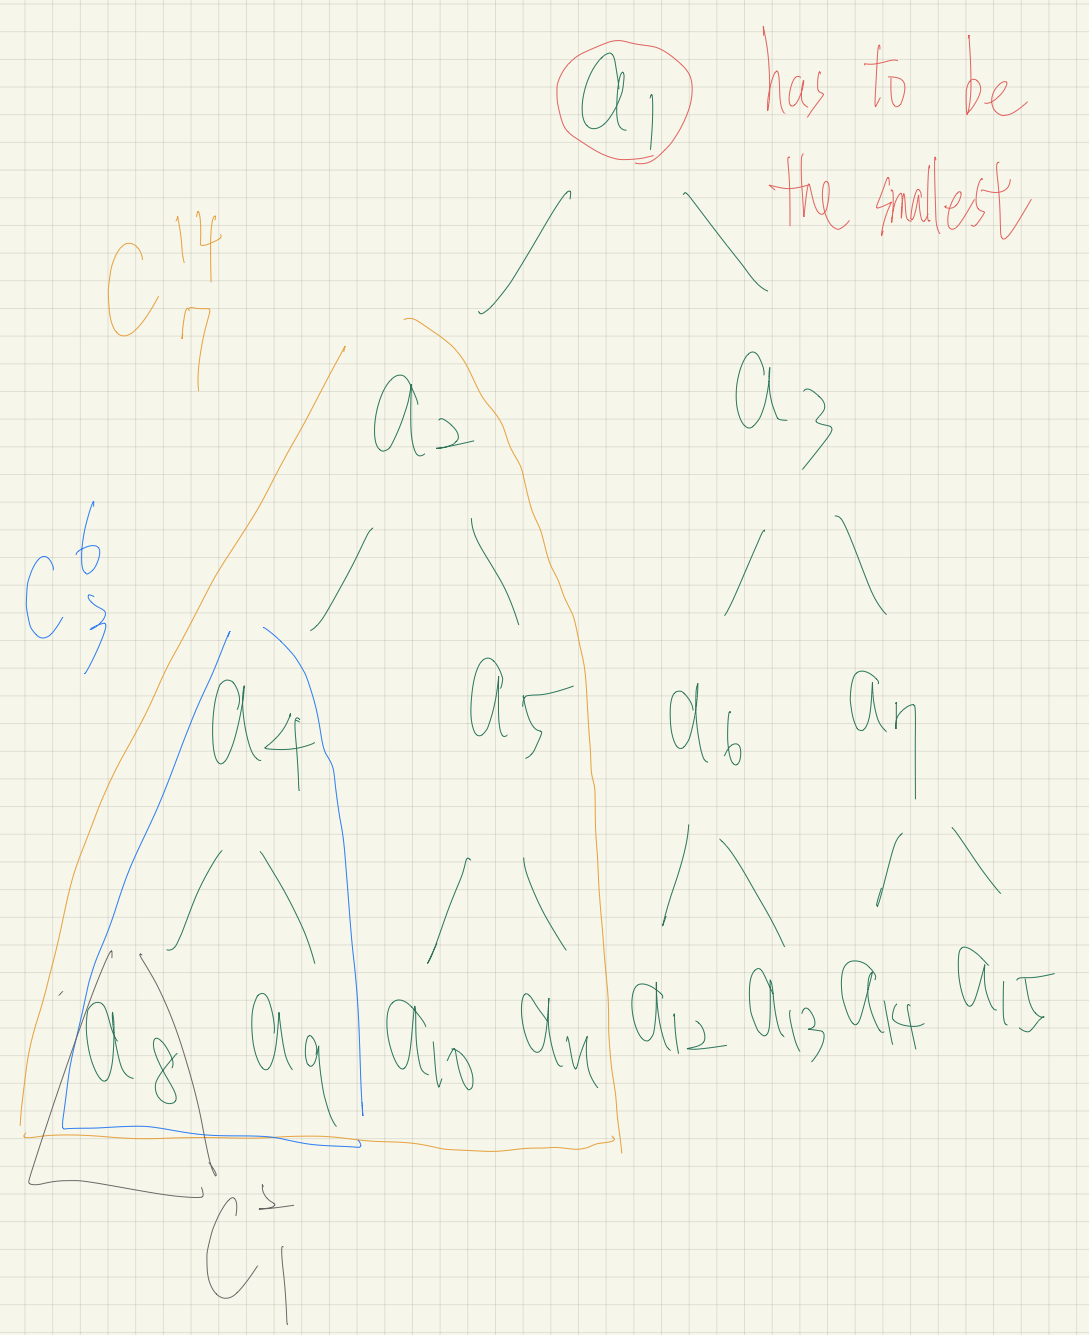
\includegraphics[width=0.6\textwidth]{IMG_0259.jpg}
            \caption{Min Heap Possibilities}
            \label{fig:my_label}
        \end{figure}
        \begin{enumerate}
            \item The root of the heap, which is arr[1] must be the smallest element.
            \item The left subtree and the right subtree are not dependent, thus we can distribute the 14 remaining elements into two groups randomly. (Causing $C^{14}_7$ possibilities)
            \item The root of each subtree has to be the smallest element of each group.
            \item Following (b), the remaining 6 (7-1) elements can be split into two groups randomly. But there are two sides needed to be calculated.(Causing $C^{6}_3 * C^{6}_3$ possibilities)
            \item Following (a) to (d), we can get the last part of the calculation as $C^{2}_1 * C^{2}_1 * C^{2}_1 * C^{2}_1$ possibilities
            \item Overall we get $C^{14}_7 * C^{6}_3 * C^{6}_3 * C^{2}_1 * C^{2}_1 * C^{2}_1 * C^{2}_1$ possibilities.
        \end{enumerate}

    \item \begin{enumerate}
        \item A possible arrangements to reach the maximum number of inverse pairs is [1,9,2,13,10,6,3,15,14,12,11,8,7,5,4], and the maximum number is $ 7+9+6+3 + C^{8}_2 = 53$
        \item The main principle to place the elements is to place the larger elements as left as possible.(Possible implies that we need to ensure all node in its (the node where we placed) subtree is larger. 
        \item The principle can imply that we achieved the arrangement that we are larger than all siblings and their subtree. Therefore, the maximum pairs is to count the elements that have lower or same level as them but are not its offspring.
    \end{enumerate} 
    

    \item  Consider the concept of Huffman's tree, we can view the direct level as its frequency.
    Then, we can directly use the Huffman's algorithm in the textbook
    \begin{enumerate}
        \item 
        \begin{algorithm} [H]
        \caption{Huffman(level)}
        \begin{algorithmic}
        \State n = $|level|$ \Comment{n = level.length}
        \State Q = level \Comment{Build a min heap}
        \For{i = 1 to n-1}
            \State Allocate a new node z
            \State z.left = x = Extract\_Min(Q)
            \State z.right = y = Extract\_Min(Q) \Comment{Finding the two materials with the least levels}
            \State z.level = x.level + y.level  \Comment{similar to the operation of fusing the material}
            \State Insert(Q,z)
        \EndFor
        \State \Return Extract\_Min(Q)
        \end{algorithmic}
        \end{algorithm}
        
        \item The time complexity is O(n) for building the min heap. The time complexity of the following loop is Extract\_Min times n loop which is n*O($log{n}) = O(nlog{n})$. Hence, the total time complexity is $ O(nlog{n})$ 

        \item The extra space complexity is O(1) because the min heap can utilize the space of the original array because there is no need to store the original array in the algorithm.
    \end{enumerate}

    \item 
        \begin{enumerate}
            \item Collect all elements with largest strength of each guild (collect origin[i][0],for i = 1 to m) and build a max heap from those elements.
            \item Also, the nodes stored in the heap must also record which guild it is from (store the row index)
            \item do extract\_max(heap) and see which guild it is from. Then insert the next largest from that guild to the heap.
            \item Until the remaining elements are less than m. We can just do m times of extract\_max(heap)
            \item Time complexity: building max heap is O(m). And we will do O(m(n-2)) inserts to the heap requiring time complexity O(m(n-2)$log{m}$) = O(mn$log{m}$)
            \item Space complexity: The max heap requires space complexity O(m).
        \end{enumerate}
\end{enumerate}

\end{CJK*}
\end{document}
